\documentclass[10pt,oneside]{article}
\usepackage[T1]{fontenc}
\usepackage[utf8]{inputenc}
% \usepackage{lmodern}
%\usepackage[adobe-utopia,uppercase=upright,greeklowercase=upright]{mathdesign}
\usepackage[adobe-utopia]{mathdesign}
%\usepackage{minionpro}
% \usepackage{pifont}
% \usepackage{amssymb}
\usepackage{amsmath}
\usepackage[francais]{babel}
% \usepackage[francais]{varioref}
\usepackage[dvips]{graphicx}

\usepackage{framed}
\usepackage[normalem]{ulem}
\usepackage{fancyhdr}
\usepackage{titlesec}
\usepackage{vmargin}
\usepackage{longtable}

\usepackage{ifthen}


%\usepackage{epsfig}
\usepackage{subfig}

\usepackage{multirow}
\usepackage{multicol} % Portions de texte en colonnes
\usepackage{flafter}%floatants après la référence



\usepackage{color}
\usepackage{colortbl}


\definecolor{gris25}{gray}{0.75}
\definecolor{bleu}{RGB}{18,33,98}
\definecolor{bleuf}{RGB}{42,94,171}
\definecolor{bleuc}{RGB}{231,239,247}
\definecolor{rougef}{RGB}{185,18,27}
\definecolor{rougec}{RGB}{255,230,231}
\definecolor{vertf}{RGB}{103,126,82}
\definecolor{vertc}{RGB}{220,255,191}
\definecolor{violetf}{RGB}{112,48,160}
\definecolor{violetc}{RGB}{230,224,236}

\newenvironment{sci}[1][\hsize]%
{%
    \def\FrameCommand%
    {%
%\rotatebox{90}{\textit{\textsf{Scilab}}\includegraphics[height=.8cm]{png/logo_scilab}} 
\rotatebox{90}{\includegraphics[height=.6cm]{png/logo_scilab}} 
        {\color{violetf}\vrule width 3pt}%
        \hspace{0pt}%must no space.
        \fboxsep=\FrameSep\colorbox{violetc}%
    }%
    \MakeFramed{\hsize #1 \advance\hsize-\width\FrameRestore}%
}%
{\endMakeFramed}%

\newenvironment{pseudo}[1][\hsize]%
{%
    \def\FrameCommand%
    {%
\rotatebox{90}{\textit{\textsf{Pseudo Code}}} 
        {\color{violetf}\vrule width 3pt}%
        \hspace{0pt}%must no space.
        \fboxsep=\FrameSep\colorbox{violetc}%
    }%
    \MakeFramed{\hsize #1 \advance\hsize-\width\FrameRestore}%
}%
{\endMakeFramed}%

\newenvironment{py}[1][\hsize]%
{%
    \def\FrameCommand%
    {%
%\rotatebox{90}{\textit{\textsf{Python}}} 
\rotatebox{90}{\includegraphics[height=.6cm]{png/logo_python}} 
        {\color{violetf}\vrule width 3pt}%
        \hspace{0pt}%must no space.
        \fboxsep=\FrameSep\colorbox{violetc}%
    }%
    \MakeFramed{\hsize #1 \advance\hsize-\width\FrameRestore}%
}%
{\endMakeFramed}%


\newenvironment{corrige}[1][\hsize]%
{%
    \def\FrameCommand
    {%
\rotatebox{90}{\textit{\textsf{Correction}}} 
        {\color{violetf}\vrule width 3pt}%
        \hspace{0pt}%must no space.
        \fboxsep=\FrameSep\colorbox{violetc}%
    }%
    \MakeFramed{\hsize#1\advance\hsize-\width\FrameRestore}%
}%
{\endMakeFramed}%



\newenvironment{rem}[1][\hsize]%
{%
    \def\FrameCommand
    {%
\rotatebox{90}{\textit{\textsf{Remarque}}} 
        {\color{bleuf}\vrule width 3pt}%
        \hspace{0pt}%must no space.
        \fboxsep=\FrameSep\colorbox{bleuc}%
    }%
    \MakeFramed{\hsize#1\advance\hsize-\width\FrameRestore}%
}%
{\endMakeFramed}%


\newenvironment{savoir}[1][\hsize]%
{%
    \def\FrameCommand
    {%
\rotatebox{90}{\textit{\textsf{Savoir}}} 
        {\color{bleuf}\vrule width 3pt}%
        \hspace{0pt}%must no space.
        \fboxsep=\FrameSep\colorbox{bleuc}%
    }%
    \MakeFramed{\hsize#1\advance\hsize-\width\FrameRestore}%
}%
{\endMakeFramed}%

\newenvironment{prob}[1][\hsize]%
{%
    \def\FrameCommand%
    {%
\rotatebox{90}{\textit{\textsf{ Problématique}}} 
        {\color{rougef}\vrule width 3pt}%
        \hspace{0pt}%must no space.
        \fboxsep=\FrameSep\colorbox{rougec}%
    }%
    \MakeFramed{\hsize#1\advance\hsize-\width\FrameRestore}%
}%
{\endMakeFramed}%

\newenvironment{obj}[1][\hsize]%
{%
    \def\FrameCommand%
    {%
\rotatebox{90}{\textit{\textsf{ $\;$}}} 
        {\color{rougef}\vrule width 3pt}%
        \hspace{0pt}%must no space.
        \fboxsep=\FrameSep\colorbox{rougec}%
    }%
    \MakeFramed{\hsize#1\advance\hsize-\width\FrameRestore}%
}%
{\endMakeFramed}%

\newenvironment{defi}[1][\hsize]%
{%
    \def\FrameCommand%
    {%
\rotatebox{90}{\textit{\textsf{Définition\\}}} 
        {\color{bleuf}\vrule width 3pt}%
        \hspace{0pt}%must no space.
        \fboxsep=\FrameSep\colorbox{bleuc}%
    }%
    \MakeFramed{\hsize#1\advance\hsize-\width\FrameRestore}%
}%
{\endMakeFramed}%


\newenvironment{demo}[1][\hsize]%
{%
    \def\FrameCommand%
    {%
\rotatebox{90}{\textit{\textsf{Démonstration\\}}} 
        {\color{bleuf}\vrule width 3pt}%
        \hspace{0pt}%must no space.
        \fboxsep=\FrameSep\colorbox{bleuc}%
    }%
    \MakeFramed{\hsize#1\advance\hsize-\width\FrameRestore}%
}%
{\endMakeFramed}%


\newenvironment{hypo}[1][\hsize]%
{%
    \def\FrameCommand%
    {%
\rotatebox{90}{\textit{\textsf{Hypothèse\\}}} 
        {\color{bleuf}\vrule width 3pt}%
        \hspace{0pt}%must no space.
        \fboxsep=\FrameSep\colorbox{bleuc}%
    }%
    \MakeFramed{\hsize#1\advance\hsize-\width\FrameRestore}%
}%
{\endMakeFramed}%


\newenvironment{prop}[1][\hsize]%
{%
    \def\FrameCommand%
    {%
\rotatebox{90}{\textit{\textsf{Propriété\\}}} 
        {\color{bleuf}\vrule width 3pt}%
        \hspace{0pt}%must no space.
        \fboxsep=\FrameSep\colorbox{bleuc}%
    }%
    \MakeFramed{\hsize#1\advance\hsize-\width\FrameRestore}%
}%
{\endMakeFramed}%

\newenvironment{props}[1][\hsize]%
{%
    \def\FrameCommand%
    {%
\rotatebox{90}{\textit{\textsf{Propriétés\\}}} 
        {\color{bleuf}\vrule width 3pt}%
        \hspace{0pt}%must no space.
        \fboxsep=\FrameSep\colorbox{bleuc}%
    }%
    \MakeFramed{\hsize#1\advance\hsize-\width\FrameRestore}%
}%
{\endMakeFramed}%

\newenvironment{exemple}[1][\hsize]%
{%
    \def\FrameCommand%
    {%
\rotatebox{90}{\textit{\textsf{Exemple\\}}} 
        {\color{vertf}\vrule width 3pt}%
        \hspace{0pt}%must no space.
        \fboxsep=\FrameSep\colorbox{vertc}%
    }%
    \MakeFramed{\hsize#1\advance\hsize-\width\FrameRestore}%
}%
{\endMakeFramed}%

\newenvironment{resultat}[1][\hsize]%
{%
    \def\FrameCommand%
    {%
\rotatebox{90}{\textit{\textsf{Résultat\\}}} 
        {\color{rougef}\vrule width 3pt}%
        \hspace{0pt}%must no space.
        \fboxsep=\FrameSep\colorbox{rougec}%
    }%
    \MakeFramed{\hsize#1\advance\hsize-\width\FrameRestore}%
}%
{\endMakeFramed}%

\newenvironment{methode}[1][\hsize]%
{%
    \def\FrameCommand%
    {%
\rotatebox{90}{\textit{\textsf{Méthode\\}}} 
        {\color{rougef}\vrule width 3pt}%
        \hspace{0pt}%must no space.
        \fboxsep=\FrameSep\colorbox{rougec}%
    }%
    \MakeFramed{\hsize#1\advance\hsize-\width\FrameRestore}%
}%
{\endMakeFramed}%

\newenvironment{theo}[1][\hsize]%
{%
    \def\FrameCommand%
    {%
\rotatebox{90}{\textit{\textsf{Théorème\\}}} 
        {\color{rougef}\vrule width 3pt}%
        \hspace{0pt}%must no space.
        \fboxsep=\FrameSep\colorbox{rougec}%
    }%
    \MakeFramed{\hsize#1\advance\hsize-\width\FrameRestore}%
}%
{\endMakeFramed}%

\newenvironment{warn}[1][\hsize]%
{%
    \def\FrameCommand%
    {%
\rotatebox{90}{\textit{\textsf{Attention\\}}} 
        {\color{rougef}\vrule width 3pt}%
        \hspace{0pt}%must no space.
        \fboxsep=\FrameSep\colorbox{rougec}%
    }%
    \MakeFramed{\hsize#1\advance\hsize-\width\FrameRestore}%
}%
{\endMakeFramed}%

% \usepackage{pstricks}
%\usepackage{minitoc}
% \setcounter{minitocdepth}{4}

\setcounter{tocdepth}{2}

% \mtcselectlanguage{french} 

%\usepackage{draftcopy}% "Brouillon"
% \usepackage{floatflt}
\usepackage{psfrag}
%\usepackage{listings} % Permet d'insérer du code de programmation
\renewcommand{\baselinestretch}{1.2}

% Changer la numérotation des figures :
% ------------------------------------
% \makeatletter
% \renewcommand{\thefigure}{\ifnum \c@section>\z@ \thesection.\fi
%  \@arabic\c@figure}
% \@addtoreset{figure}{section}
% \makeatother
 


%%%%%%%%%%%%
% Définition des vecteurs %
%%%%%%%%%%%%
 \newcommand{\vect}[1]{\overrightarrow{#1}}

%%%%%%%%%%%%
% Définition des torseusr %
%%%%%%%%%%%%

 \newcommand{\torseur}[1]{%
\left\{{#1}\right\}
}

\newcommand{\torseurcin}[3]{%
\left\{\mathcal{#1} \left(#2/#3 \right) \right\}
}

\newcommand{\torseurstat}[3]{%
\left\{\mathcal{#1} \left(#2\rightarrow #3 \right) \right\}
}

 \newcommand{\torseurc}[8]{%
%\left\{#1 \right\}=
\left\{
{#1}
\right\}
 = 
\left\{%
\begin{array}{cc}%
{#2} & {#5}\\%
{#3} & {#6}\\%
{#4} & {#7}\\%
\end{array}%
\right\}_{#8}%
}

 \newcommand{\torseurcol}[7]{
\left\{%
\begin{array}{cc}%
{#1} & {#4}\\%
{#2} & {#5}\\%
{#3} & {#6}\\%
\end{array}%
\right\}_{#7}%
}

 \newcommand{\torseurl}[3]{%
%\left\{\mathcal{#1}\right\}_{#2}=%
\left\{%
\begin{array}{l}%
{#1} \\%
{#2} %
\end{array}%
\right\}_{#3}%
}

 \newcommand{\vectv}[3]{%
\vect{V\left( {#1} \in {#2}/{#3}\right)}
}


\newcommand{\vectf}[2]{%
\vect{R\left( {#1} \rightarrow {#2}\right)}
}

\newcommand{\vectm}[3]{%
\vect{\mathcal{M}\left( {#1}, {#2} \rightarrow {#3}\right)}
}


 \newcommand{\vectg}[3]{%
\vect{\Gamma \left( {#1} \in {#2}/{#3}\right)}
}

 \newcommand{\vecto}[2]{%
\vect{\Omega\left( {#1}/{#2}\right)}
}
% }$$\left\{\mathcal{#1} \right\}_{#2} =%
% \left\{%
% \begin{array}{c}%
%  #3 \\%
%  #4 %
% \end{array}%
% \right\}_{#5}}

%  ------------------------------------------
% | Modification du formatage des sections : | 
%  ------------------------------------------

% Grands titres :
% ---------------

\newcommand{\titre}[1]{%
\begin{center}
      \bigskip
      \rule{\textwidth}{1pt}
      \par\vspace{0.1cm}
      
      \textbf{\large #1}
      \par\rule{\textwidth}{1pt}
    \end{center}
    \bigskip
  }

% Supprime le numéro du chapitre dans la numérotation des sections:
% -----------------------------------------------------------------
\makeatletter
\renewcommand{\thesection}{\@arabic\c@section}
\makeatother


% \titleformat{\chapter}[display]
% {\normalfont\Large\filcenter}
% {}
% {1pc}
% {\titlerule[1pt]
%   \vspace{1pc}%
%   \Huge}[\vspace{1ex}%
% \titlerule]


%%%% Chapitres Comme PY Pechard %%%%%%%%%
% numéro du chapitre
\DeclareFixedFont{\chapnumfont}{OT1}{phv}{b}{n}{80pt}
% pour le mot « Chapitre »
\DeclareFixedFont{\chapchapfont}{OT1}{phv}{m}{it}{40pt}
% pour le titre
\DeclareFixedFont{\chaptitfont}{T1}{phv}{b}{n}{25pt}

\definecolor{gris}{gray}{0.75}
\titleformat{\chapter}[display]%
	{\sffamily}%
	{\filleft\chapchapfont\color{gris}\chaptertitlename\
	\\
	\vspace{12pt}
	\chapnumfont\thechapter}%
	{16pt}%
	{\filleft\chaptitfont}%
	[\vspace{6pt}\titlerule\titlerule\titlerule]

%%%%  Fin Chapitres Comme PY Pechard %%%%%%%%%


% Section, subsection, subsubsection sans serifs :
% % ----------------------------------------------

% \makeatletter
% \renewcommand{\section}{\@startsection{section}{0}{0mm}%
% {\baselineskip}{.3\baselineskip}%
% {\normalfont\sffamily\Large\textbf}}%
% \makeatother

\makeatletter
\renewcommand{\@seccntformat}[1]{{\textcolor{bleu}{\csname
the#1\endcsname}\hspace{0.5em}}}
\makeatother

\makeatletter
\renewcommand{\section}{\@startsection{section}{1}{\z@}%
                       {-4ex \@plus -1ex \@minus -.4ex}%
                       {1ex \@plus.2ex }%
                       {\normalfont\Large\sffamily\bfseries}}%
\makeatother
 
\makeatletter
\renewcommand{\subsection}{\@startsection {subsection}{2}{\z@}
                          {-3ex \@plus -0.1ex \@minus -.4ex}%
                          {0.5ex \@plus.2ex }%
                          {\normalfont\large\sffamily\bfseries}}
\makeatother
 
\makeatletter
\renewcommand{\subsubsection}{\@startsection {subsubsection}{3}{\z@}
                          {-2ex \@plus -0.1ex \@minus -.2ex}%
                          {0.2ex \@plus.2ex }%
                          {\normalfont\large\sffamily\bfseries}}
\makeatother
 
\makeatletter             
\renewcommand{\paragraph}{\@startsection{paragraph}{4}{\z@}%
                                    {-2ex \@plus-.2ex \@minus .2ex}%
                                    {0.1ex}%               
{\normalfont\sffamily\bfseries}}
\makeatother
 

\makeatletter             
\renewcommand{\subparagraph}{\@startsection{subparagraph}{5}{\z@}%
                                    {-2ex \@plus-.2ex \@minus .2ex}%
                                    {0.1ex}%               
{\normalfont\bfseries Question }}
\makeatother

\renewcommand{\thesubparagraph}{\arabic{subparagraph}} 
%
\makeatletter
%\renewcommand{\subparagraph}{\@startsection{subparagraph}{5}{\z@}%
%                                       {-2ex \@plus-.1ex \@minus .2ex}%
%                                       {0.1ex}%
%				    {\normalfont\normalsize\sffamily\bfseries}}
%\makeatletter
% \makeatletter
% \renewcommand{\subsection}{\@startsection{subsection}{1}{2mm}%
% {\baselineskip}{.3\baselineskip}%
% {\normalfont\sffamily\large\textbf}}%
% \makeatother
% 
% \makeatletter
% \renewcommand{\subsubsection}{\@startsection{subsubsection}{2}{4mm}%
% {\baselineskip}{.15\baselineskip}%
% {\normalfont\sffamily\large\textbf}}%
% \makeatother
% 
% \makeatletter
% \renewcommand{\paragraph}{\@startsection{paragraph}{3}{6mm}%
% {\baselineskip}{.15\baselineskip}%
% {\normalfont\sffamily\large\textbf}}%
% \makeatother
 
\setcounter{secnumdepth}{5}


%  --------
% | Marges |
%  --------


% \setmarginsrb{2.5cm}{1.5cm}{2.5cm}{2cm}{1cm}{1cm}{1cm}{1cm}
\setmarginsrb{1.5cm}{1cm}{1cm}{1.5cm}{1cm}{1cm}{1cm}{1cm}

% Changer les marges localement :
% -----------------------------
\newenvironment{changemargin}[2]{\begin{list}{}{%
\setlength{\topsep}{0pt}%
\setlength{\leftmargin}{0pt}%
\setlength{\rightmargin}{0pt}%
\setlength{\listparindent}{\parindent}%
\setlength{\itemindent}{\parindent}%
\setlength{\parsep}{0pt plus 1pt}%
\addtolength{\leftmargin}{#1}%
\addtolength{\rightmargin}{#2}%
}\item }{\end{list}}



\usepackage{pst-solides3d}
\usepackage{titletoc}
\titlecontents{chapter}[+3pc]
  {\addvspace{10pt}\sffamily\bfseries}
{\contentslabel[{\pscirclebox[fillstyle=solid,fillcolor=gray!25,
linecolor=gray!25,framesep=4pt]{\textcolor{white}{\thecontentslabel}}}]{2.5pc}}
  {}
  {\dotfill \normalfont\thecontentspage\ }

\titlecontents{section}[3pc]
  {\addvspace{2pt}\sffamily}
  {\contentslabel[\thecontentslabel]{1.8pc}}
  {}
  {\dotfill \normalfont\thecontentspage\ }

\titlecontents{subsection}[5pc]
  {\addvspace{2pt}\sffamily}
  {\contentslabel[\thecontentslabel]{1.8pc}}
  {}
  {\dotfill \normalfont\thecontentspage\ }

\titlecontents{subsubsection}[8pc]
  {\addvspace{2pt}\sffamily}
  {\contentslabel[\thecontentslabel]{3pc}}
  {}
  {\dotfill \normalfont\thecontentspage\ }
%{\;\titlerule\;\normalfont\thecontentspage\ }

\titlecontents{paragraph}[9pc]
  {\addvspace{2pt}\sffamily}
  {\contentslabel[\thecontentslabel]{3.5pc}}
  {}
  {\dotfill \normalfont\thecontentspage\ }




\usepackage[%
    pdftitle={CIN -- Torseurs -- Travaux Dirigés},
    pdfauthor={Xavier Pessoles},
    colorlinks=true,
    linkcolor=blue,
    citecolor=magenta]{hyperref}



% \makeatletter \let\ps@plain\ps@empty \makeatother
%% DEBUT DU DOCUMENT
%% =================
\sloppy
\hyphenpenalty 10000

\newcommand{\Pointilles}[1][3]{%
\multido{}{#1}{\makebox[\linewidth]{\dotfill}\\[\parskip]
}}


\begin{document}


\newboolean{prof}
\setboolean{prof}{false}
%------------- En tetes et Pieds de Pages ------------
\pagestyle{fancy}
\renewcommand{\headrulewidth}{0pt}

\fancyhead{}
\fancyhead[L]{%
\noindent\noindent\begin{minipage}[c]{2.6cm}
%Lycée Rouvière PTSI
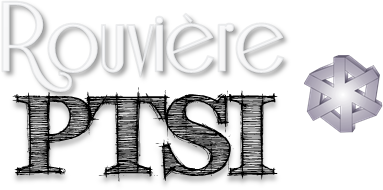
\includegraphics[width=2cm]{png/logo_ptsi.png}%
\end{minipage}
}

\fancyhead[C]{\rule{12cm}{.5pt}}

\fancyhead[R]{%
\begin{minipage}[c]{3cm}
\begin{flushright}
\footnotesize{\textit{\textsf{Sciences Industrielles\\ de l'Ingénieur}}}%
\end{flushright}
\end{minipage}
}

\renewcommand{\footrulewidth}{0.2pt}

\fancyfoot[C]{\footnotesize{\bfseries \thepage}}
\fancyfoot[L]{\footnotesize{2013 -- 2014} \\ X. \textsc{Pessoles}}
\ifthenelse{\boolean{prof}}{%
\fancyfoot[R]{\footnotesize{CI 3 : CIN -- TD} \\ \footnotesize{Ch 7 : Torseurs -- P}}
}{%
\fancyfoot[R]{\footnotesize{CI 3 : CIN -- TD} \\ \footnotesize{Ch 7 : Torseurs -- E}}
}


%\begin{center}
%\textit{Centre d'intérêt}
%\end{center}



\begin{center}
 \Large\textsc{CI 3 -- CIN : Étude du comportement cinématique des systèmes}
\end{center}

\begin{center}
 \large\textsc{Chapitre 7 -- Torseurs}
\end{center}

\begin{center}
\textsc{Travaux Dirigés} 
\end{center}

\vspace{.5cm}

\subsection*{Exercice 1 -- Came plate}
\setcounter{subparagraph}{0}
\begin{flushright}
\textit{D'après ressources de Jean-Pierre Pupier.} 
\end{flushright}
La came plate 1 tourne et transmet un mouvement de translation alternatif à la pièce 2. Il y a une liaison sphère -- plan de centre A.

\begin{itemize}
\item On associe au bâti 0 un repère $\mathcal{R}_0=\left(H,\vect{x_0},\vect{y_0},\vect{z_0}, \right)$.
\item On associe à la came plate 1 un repère  $\mathcal{R}_1=\left(H,\vect{x_0},\vect{y_1},\vect{z_1} \right)$. 
\item On pose  $\alpha=\left( \vect{y_0}, \vect{y_1}\right)$.
\item Un repère $\mathcal{R}'_1$ est également lié à 1 : $\mathcal{R}'_1=\left(H,\vect{x'_1},\vect{y'_1},\vect{z_1} \right)$. 
\item Ce repère est tel que $\vect{x'_1}$ est perpendiculaire à la surface plane de 1 sur laquelle appuie la sphère.
\item On pose $\theta= \left( \vect{x_0}, \vect{x'_1}\right)$. $\theta$ est constant.
\item On associe à la pièce 2 un repère  $\mathcal{R}_2=\left(A,\vect{x_0},\vect{y_0},\vect{z_0} \right)$. 
\item On pose $\vect{HA}=R\vect{y_0}+\lambda\vect{x_0}$ où $R$ est constant et $\lambda$ variable.
\end{itemize}

\begin{center}
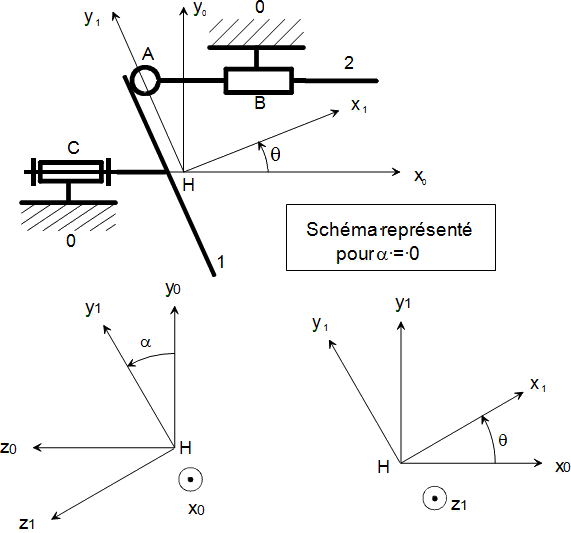
\includegraphics[width=.6\textwidth]{png/fig_01}
\end{center}

\subparagraph{}
\textit{Exprimer les torseurs $\torseur{\mathcal{V}(1/0)}$ et $\torseur{\mathcal{V}(2/0)}$. Préciser les noms de ces deux types de torseurs.}
\ifthenelse{\boolean{prof}}{
\begin{corrige}
Les solides 1 et 0 sont en liaison pivot de centre $C$ et d'axe $(A,\vect{x_0})$. En conséquence, on a: 
$$
\torseur{\mathcal{V}(1/0)} =
\torseurl{\vecto{1}{0}=\dot{\alpha}\vect{x_0}}{\vectv{C}{1}{0}=\vect{0}}{C,\mathcal{R}_0}
$$

Les solides 2 et 0 sont en liaison glissière d'axe $\vect{x_0}$. En conséquence, on a: 
$$
\torseur{\mathcal{V}(2/0)} =
\torseurl{\vecto{2}{0}=\vect{0}}{\vectv{B}{2}{0}=\dot{\lambda}\vect{x_0}}{C,\mathcal{R}_0}
$$

Le torseur $\torseur{\mathcal{V}(1/0)}$ est un glisseur.

Le torseur $\torseur{\mathcal{V}(2/0)}$ est un couple.

\end{corrige}
}{}

\subparagraph{}
\textit{Exprimer le torseur $\torseur{\mathcal{V}(2/1)}$.}
\ifthenelse{\boolean{prof}}{

\begin{corrige}
Les solides 2 et 1 sont en liaison ponctuelle d'axe $(A,\vect{x'_1})$. En conséquence, on a: 
$$
\torseur{\mathcal{V}(2/1)} =
\torseurl{\vecto{2}{1}=\omega_x \vect{x'_1}+\omega_y \vect{y'_1} + \omega_z \vect{z_1} }{\vectv{A}{2}{1}=v_y\vect{y'_1}+v_z\vect{z'_1}}{A,\mathcal{R}'_1}
$$
\end{corrige}
}{}


\subparagraph{}
\textit{Trouver la relation entre $\dot{\lambda}$ et $\dot{\alpha}$.}
\ifthenelse{\boolean{prof}}{
\begin{corrige}
D'après la composition du torseur cinématique, on a :
$$
\torseur{\mathcal{V}(2/1)} = \torseur{\mathcal{V}(2/0)} + \torseur{\mathcal{V}(0/1)} \Longleftrightarrow 
\torseur{\mathcal{V}(2/1)} = \torseur{\mathcal{V}(2/0)} - \torseur{\mathcal{V}(1/0)}
$$

Afin d'utiliser la relation de décomposition, il est nécessaire d'exprimer les torseurs au même point. Choisissons le point $A$ : 
\begin{eqnarray*}
\vectv{A}{2}{0} &=& \vectv{B}{2}{0}  + \vect{AB}\wedge\vecto{2}{0} \\
& = &  \vectv{B}{2}{0}   = \dot{\lambda}\vect{x_0} \text{ car } \vecto{2}{0} = \vect{0}
\end{eqnarray*}

Par ailleurs, 

\begin{eqnarray*}
\vectv{A}{1}{0} &=& \vectv{C}{1}{0}  + \vect{AC}\wedge\vecto{1}{0} \\
& = &  \left( -R \vect{y_0} - \lambda \vect{x_0}- L\vect{x_0} + \right) \wedge \dot{\alpha}\vect{x_0} \\
 & = & R \dot{\alpha}\vect{z_0}
\end{eqnarray*}

On a donc :
$$
\vectv{A}{2}{1}=\vectv{A}{2}{0}-\vectv{A}{1}{0} = \dot{\lambda}\vect{x_0}  - R \dot{\alpha}\vect{z_0}
$$

Projetons $\vectv{A}{2}{1}$ dans $\mathcal{R}'_1$ :
\begin{itemize}
\item [$\bullet$] $\vect{x_0} =\vect{x_1}=\cos\theta \vect{x'_1} -\sin\theta \vect{y'_1}$;
\item [$\bullet$] $\vect{z_0} =\cos\alpha \vect{z_1} +\sin\alpha \vect{y_1}
=\sin\alpha \sin\theta \vect{x'_1}+\sin\alpha\cos\theta \vect{y'_1} + \cos\alpha \vect{z'_1} $.
\end{itemize}

D'où :
$$
\vectv{A}{2}{1}= \dot{\lambda}\left(\cos\theta \vect{x'_1} -\sin\theta \vect{y'_1}\right)  - R \dot{\alpha}\left( \sin\alpha \sin\theta \vect{x'_1}+\sin\alpha\cos\theta \vect{y'_1} + \cos\alpha \vect{z'_1}\right)
$$

D'après la question précédente, $\vectv{A}{2}{1}\cdot\vect{x'_1}= 0$. Au final, 
$$
\dot{\lambda}\cos\theta  - R \dot{\alpha} \sin\alpha \sin\theta =0 
\Longleftrightarrow
\dot{\lambda}\cos\theta  = R \dot{\alpha} \sin\alpha \sin\theta 
\Longleftrightarrow
\dot{\lambda}  = R \dot{\alpha} \sin\alpha \tan\theta 
$$
\end{corrige}
}{}


\subparagraph{}
\textit{Trouver l'expression de $\lambda$ et exprimer la course de 2 par rapport à 0. }
\ifthenelse{\boolean{prof}}{
\begin{corrige}
En intégrant l'expression précédente, on a : $\lambda  =- R \cos\alpha \tan\theta + k
$ avec $k$ constante. En conséquence, lorsque $\alpha=0$ alors $\lambda=-R\tan\theta + k$. Or, d'après la modélisation, lorsque $\alpha=0$,$\lambda = -R\tan\theta$. On a donc $k=0$ et :
$$
\lambda(t)=-R\cos\alpha(t)\tan\theta
$$

La pièce 2 parcourt sa course complète lorsque $\alpha$ varie de $0$ à $\pi$. On a donc : 
$$
c = |\lambda(\pi)-\lambda(0)| = |-R\tan\theta - R\tan\theta| = 2R\tan\theta
$$
\end{corrige}
}{}

\subparagraph{}
\textit{Trouver la vitesse de glissement $\vectv{A}{2}{1}$ dans $\mathcal{B}'_1$ sans faire intervenir $\lambda$ (et sa dérivée).}
\ifthenelse{\boolean{prof}}{
\begin{corrige}
On a vu que : 
$$
\vectv{A}{2}{1}= -\dot{\lambda} \sin\theta \vect{y'_1}  - R \dot{\alpha}\sin\alpha\cos\theta \vect{y'_1} - R \dot{\alpha} \cos\alpha \vect{z'_1}
$$
En utilisant la question 3, on a :
\begin{eqnarray*}
\vectv{A}{2}{1}&=& - R \dot{\alpha} \sin\alpha \tan\theta  \sin\theta \vect{y'_1}  - R \dot{\alpha}\sin\alpha\cos\theta \vect{y'_1} - R \dot{\alpha} \cos\alpha \vect{z'_1} \\
\end{eqnarray*}
\end{corrige}
}{}


\end{document}
\setcounter{subparagraph}{0}

\subparagraph{}
\textit{}
\ifthenelse{\boolean{prof}}{
\begin{corrige}
\end{corrige}
}{}
